\documentclass[11pt,a4paper]{amsart}
\usepackage[T1]{fontenc}
\usepackage{lmodern}
\usepackage[a4paper,margin=26mm]{geometry}
\usepackage{amsmath,amssymb,amsthm,booktabs,microtype,graphicx}
\usepackage[hidelinks]{hyperref}
\usepackage{xurl}
\usepackage{needspace}
\usepackage[foot]{amsaddr}
\newtheorem{theorem}{Theorem}[section]
\newtheorem{proposition}[theorem]{Proposition}
\newtheorem{lemma}[theorem]{Lemma}
\newtheorem{corollary}[theorem]{Corollary}
\theoremstyle{definition}\newtheorem{definition}[theorem]{Definition}
\DeclareMathOperator{\lcm}{lcm}
\DeclareMathOperator{\li}{li}
\newcommand{\kap}{\kappa_M}
\newcommand{\EE}{\mathcal E}
\newcommand{\NN}{\mathbb N}
\newcommand{\eps}{\varepsilon}
\hypersetup{pdfauthor={Deep Bhattacharjee, Tristan Romanov, Ushashi Bhattacharya},
 pdftitle={Stronger Sieve Bounds and Complete Type I Source Searches for the Erdos-Straus Equation}}
\title[Type I source searches for the Erd\H{o}s--Straus equation]{Stronger sieve bounds and complete Type~I source searches for the Erd\H{o}s--Straus equation}
\author[D. Bhattacharjee]{Deep Bhattacharjee}
\address[Deep Bhattacharjee]{Formerly, Electro-Gravitational Space Propulsion Laboratory
(EGSPL), Bhubaneswar, Odisha 751030, India; Formerly, University of
Calcutta (Heramba Chandra College), 23/49 Gariahat Road, Golpark,
Kolkata 700029, West Bengal, India}
\email{egspl@proton.me}
\thanks{Corresponding author: Deep Bhattacharjee, egspl@proton.me.
ORCID: Deep Bhattacharjee,
\href{https://orcid.org/0000-0003-0466-750X}{0000-0003-0466-750X};
Ushashi Bhattacharya,
\href{https://orcid.org/0009-0002-2254-3914}{0009-0002-2254-3914}.}
\author[T. Romanov]{Tristan Romanov}
\address[Tristan Romanov]{Independent Researcher, San Francisco, CA, USA}
\author[U. Bhattacharya]{Ushashi Bhattacharya}
\address[Ushashi Bhattacharya]{Formerly, National Taiwan University, Taipei 106319, Taiwan}
\subjclass[2020]{11D68, 11N36}
\keywords{Egyptian fractions, Type I solutions, arithmetic large sieve,
search depth, reciprocal totient sums}
\date{15 November 2026}
\begin{document}
\begin{abstract}
We study failures of a Type~I source search for the Erd\H{o}s--Straus
equation. At depth $M$, the sieve exponent is
$\sum_{i\le M}1/\varphi(4i)$, with a uniform bound for
$M\le(\log X)/5$. At square-root depth, the failure count is
$O_a(Xe^{-a\sqrt{\log X}})$ for every $a<0.8049009$.
The prime $30241$ requires a source beyond this cutoff.
A complementary search in the auxiliary parameter finds every
witness in the specified family within explicit finite bounds.
Universal nonemptiness remains open.
\end{abstract}
\maketitle

\section{Introduction and results}
The Erd\H{o}s--Straus conjecture asks for positive integers $x,y,z$ with
\begin{equation}\label{eq:es}
 \frac4n=\frac1x+\frac1y+\frac1z
 \qquad(n\ge2).
\end{equation}
Scaling all denominators by $t$ carries a solution for $n$ to one for
$tn$, so the prime inputs suffice. For a prime $p\equiv3\pmod4$,
the identity with denominators
$((p+1)/4,\ p(p+1)/2,\ p(p+1)/2)$ applies.
The prime $2$ is immediate. We therefore concentrate on
$p\equiv1\pmod4$.

For $1\le i<p$, say that \emph{source $i$ succeeds} when
\begin{equation}\label{eq:source}
 d\mid p+i,\qquad d\equiv3\pmod4,\qquad 4i\mid p+d
\end{equation}
for a positive divisor $d$. Put
\[
 F_i=\{p\equiv1\pmod4\text{ prime for which source }i\text{ fails}\}.
\]
Write
\[
 E(X;M)=\#\left\{p\le X:p>M,\
                         p\in\bigcap_{i=1}^M F_i\right\}.
\]
The harmless restriction $p>M$ keeps the source terminology uniform.
Write
\[
 M(p)=\lfloor\sqrt p/2\rfloor,\qquad
 E_{\sqrt{\ }}(X)=\#\{p\le X:p\in\bigcap_{i\le M(p)}F_i\}.
\]
The parameter $M(p)$ is a specified search budget.

The two source certificates lead to complementary small-sieve and
arithmetic large-sieve estimates.\footnote{Tristan Romanov contributed
the initial source certificates and sieve analysis. The present
version also develops the distinct-block denominator estimate and
the complete complementary parameter search.}
The congruences \eqref{eq:source} are
Yamamoto's Type~I congruence family with parameter $a=1$, in the
classification of Elsholtz and Tao \cite[Proposition~1.9]{ET}.
They provide a more restricted search than the full set of
unit-fraction solutions. Dahan's two-parameter Type~II search \cite{Dahan} concerns another
witness set. Our count $E_{\sqrt{\ }}(X)$ records failure of the specified Type~I
budget, including the explicit prime in Section~\ref{sec:pointwise}.

Here and below $\log$ is natural, and constants implicit in $O_B$ or
$\ll_B$ may depend on $B$. Let
\[
 \kappa_M=\sum_{i\le M}\frac1{\varphi(4i)},\qquad
 C_*=\frac{\zeta(2)\zeta(3)}{3\zeta(6)}=0.64786548\ldots .
\]
\begin{theorem}[Fixed and logarithmic depth]\label{thm:uniform}
For fixed $M\ge1$,
\begin{equation}\label{eq:fixed}
 E(X;M)\ll_M \frac{X}{(\log X)^{1+\kappa_M}}.
\end{equation}
There is an absolute $c>0$ such that, for each $B\ge2$, a constant $K_B$
satisfies
\begin{equation}\label{eq:uniform}
 E(X;M)\le K_B\pi(X)(\log X)^{-\kappa_M}
 \exp\left(\frac{\kappa_M\log(4M)}B+
             c\kappa_M\log\log(3M)\right)
\end{equation}
uniformly for $X\ge3$ and $2\le M\le(\log X)/5$.
The constant $K_B$ can be ineffective.
\end{theorem}
\begin{corollary}\label{cor:loglog}
For every $\eps>0$,
\[
 E_{\sqrt{\ }}(X)\ll_\eps
 \pi(X)\exp(-(C_*-\eps)(\log\log X)^2).
\]
\end{corollary}

For an odd prime $f$, define
\[
 \omega(f)=\#\{m\mid f+1:m\equiv3\pmod4\},\qquad \omega(2)=0,
 \qquad
 L(Q)=\sum_{q\le Q}\mu^2(q)\prod_{f\mid q}
                       \frac{\omega(f)}{f-\omega(f)}.
\]
Empty products equal one, and products indexed by $f$ run over primes.
\begin{theorem}[Fixed residue classes]\label{thm:large}
If $I$ contains $N$ consecutive integers and $Q\ge2$, then
\[
 \#\{p\in I:p\equiv1\pmod4\text{ prime},\
       p>\lfloor(Q+1)/3\rfloor,\
       p\in\bigcap_{i\le\lfloor(Q+1)/3\rfloor} F_i\}
 \le\frac{N+Q^2}{L(Q)}.
\]
Furthermore,
\begin{equation}\label{eq:L}
 \log L(Q)\ge(\sqrt{2C_*}-o(1))\sqrt{\log Q}.
\end{equation}
Consequently, for every $0<a<\sqrt{C_*}$,
\begin{equation}\label{eq:sqrt}
 E_{\sqrt{\ }}(X)\ll_a X\exp(-a\sqrt{\log X}).
\end{equation}
\end{theorem}
The admissible threshold is $\sqrt{C_*}=0.804900912498\ldots$.
All limiting choices in this estimate are fixed before $X$ tends to infinity.

Vaughan's classical bound for actual insoluble integers has exponent
$2/3$ \cite{Vaughan}. Recent preprints report further estimates on
those exceptional integers \cite{DahanComposite,Trybushnyi}.
The failure count studied here has its own prescribed witness
family. In particular, \eqref{eq:sqrt} bounds a set that can contain
representable primes.

\section{Algebraic certificates}
\begin{lemma}[Source identity]\label{lem:identity}
Under \eqref{eq:source}, put $k=(p+d)/(4i)$ and $A=(p+i)/d$. Then
\begin{equation}\label{eq:triple}
 (x,y,z)=(ik,ikA,pkA)
\end{equation}
are positive integers satisfying \eqref{eq:es} for $n=p$.
Exactly one of them is divisible by $p$.
\end{lemma}
\begin{proof}
The numerator of the sum of unit fractions over common denominator
$pikA$ is
$pA+p+i=(p+i)(p+d)/d=4ikA$.
Also $\gcd(p,i)=1$ and $p\nmid(p+i)$.
Since $d\mid p+i$, both $d$ and $A$ are coprime to $p$.
The equation $4ik=p+d$ gives $p\nmid k$. These facts prove the last claim.
\end{proof}

\begin{lemma}[Prime and cofactor rules]\label{lem:rules}
Let $q\mid p+i$ with $q$ prime. Source $i$ succeeds if
$q\equiv-p\pmod{4i}$. It also succeeds if $i$ is even and
$q\equiv-1-i\pmod{4i}$.
The latter rule holds for composite divisors $q$ as well.
\end{lemma}
\begin{proof}
In the first case use $d=q$, since $p\equiv1\pmod4$.
For the second take $d=(p+i)/q$.
The congruence implies $\gcd(q,4i)=1$ and
\[
 q(p+d)=qp+p+i\equiv-i(p-1)\equiv0\pmod{4i}.
\]
Thus $4i\mid p+d$, which also gives $d\equiv3\pmod4$.
\end{proof}

\begin{lemma}[Classes independent of $p$]\label{lem:classes}
For an odd prime $f$ and a divisor $m\mid f+1$ with $m\equiv3\pmod4$,
set $i=(f+1)/m$. Then $i$ is even and
$2\le i\le(f+1)/3<f$. Every prime $p\equiv1\pmod4$
with $p\equiv-i\pmod f$ has source $i$ succeeding.
The $\omega(f)$ residues $-i\pmod f$ are distinct and nonzero.
\end{lemma}
\begin{proof}
Since $m$ is odd, $i$ is even. Also
$f=im-1\equiv-i-1\pmod{4i}$, so Lemma~\ref{lem:rules} applies
once $i<p$. If $p\le i$, divisibility $f\mid p+i$ would give
$0<p+i\le2i\le2(f+1)/3<f$, a contradiction for the primes
with $\omega(f)>0$. Distinct divisors give distinct
$i\in[2,(f+1)/3]$, so give distinct nonzero residues.
\end{proof}

\section{The reciprocal-totient exponent}
\begin{lemma}\label{lem:kappa}
One has $\kappa_M=C_*\log M+O(1)$.
\end{lemma}
\begin{proof}
The divisor identity
$n/\varphi(n)=\sum_{d\mid n}\mu^2(d)/\varphi(d)$ gives
\[
 \sum_{\substack{j\le x\\j\text{ odd}}}\frac1{\varphi(j)}
 =\sum_{\substack{d\le x\\d\text{ odd}}}
   \frac{\mu^2(d)}{d\varphi(d)}
   \sum_{\substack{k\le x/d\\k\text{ odd}}}\frac1k .
\]
The inner sum is $\frac12\log(x/d)+O(1)$.
The sums with coefficients $\mu^2(d)/(d\varphi(d))$, and the
same coefficients times $\log d$, converge. Their tails,
using $\varphi(d)\gg_\eps d^{1-\eps}$, justify extending
the leading coefficient to infinity with bounded error.
Its Euler product is
\[
 \frac12\prod_{\ell>2}\left(1+\frac1{\ell(\ell-1)}\right)
 =\frac13\prod_\ell\left(1+\frac1{\ell(\ell-1)}\right)=C_*.
\]
The last product equals $\zeta(2)\zeta(3)/\zeta(6)$.
Write $i=2^a j$ with $j$ odd. Since
$\varphi(4i)=2^{a+1}\varphi(j)$, summing the odd estimate
with weights $2^{-a-1}$ yields
$\kappa_M=C_*\log M+O(1)$.
\end{proof}

\section{A Selberg bound with the remainder exposed}\label{sec:selberg}
We record the finite sieve inequality used for uniformity.
Let $P$ be a product of finitely many primes. At a prime $q\mid P$
let $\Omega(q)$ have $\rho(q)$ forbidden residues with $0<\rho(q)<q$.
Put $g(q)=\rho(q)/q$ and $h(q)=g(q)/(1-g(q))$, extended
multiplicatively to squarefree integers. Suppose
\[
 |\mathcal A_d|=X'g(d)+R_d,\qquad |R_d|\le\rho(d)
\]
for squarefree $d\mid P$, with $\rho(d)=\prod_{q\mid d}\rho(q)$.
Here $\mathcal A_d$ imposes a forbidden residue at each $q\mid d$.
\begin{lemma}\label{lem:selberg}
For $\xi>1$ and $G(\xi)=\sum_{d<\xi,d\mid P}h(d)$,
the number avoiding all forbidden residues is at most
\[
 \frac{X'}{G(\xi)}
 +\sum_{\substack{d<\xi^2\\d\mid P}}3^{\nu(d)}\rho(d).
\]
\end{lemma}
\begin{proof}
Choose $\lambda_1=1$, with $\lambda_d=0$ unless $d\mid P$ and
$d<\xi$, and majorize avoidance by
$(\sum_{d}\lambda_d\mathbf1_{\mathcal A_d})^2$.
The main quadratic form is
\[
 \sum_{d_1,d_2}\lambda_{d_1}\lambda_{d_2}g([d_1,d_2])
 =\sum_l\frac1{h(l)}
       \left(\sum_{l\mid d}\lambda_d g(d)\right)^2.
\]
This follows prime by prime from $1/g(q)=1+1/h(q)$.
Writing $y_l=\sum_{l\mid d}\lambda_dg(d)$, inversion gives
$\lambda_1=\sum_l\mu(l)y_l$. Choose
$y_l=\mu(l)h(l)/G(\xi)$ for $l<\xi$ dividing $P$, and zero otherwise.
The quadratic form is then $1/G(\xi)$ and inversion gives
\[
 |\lambda_d|=
 \prod_{q\mid d}(1+h(q))\,
 \frac{\sum_{m<\xi/d,\ (m,d)=1,\ m\mid P}h(m)}{G(\xi)}
 \le1.
\]
For the inequality, the numerator is a sub-sum of $G(\xi)$
by writing the summation integer uniquely as $am$ with $a\mid d$.
For a squarefree $d$ there are $3^{\nu(d)}$ ordered pairs
$(d_1,d_2)$ with $[d_1,d_2]=d$. Bounding their remainder
contributions with $|\lambda_d|\le1$ proves the result.
\end{proof}
This is the usual Selberg quadratic-form argument
\cite[Chapter~9]{Richert}, also developed in \cite{HR}.
We include the finite form to keep its constants in $M$ visible.

\section{Proof at logarithmic depth}
Set
\[
 N_M=4\lcm(1,\ldots,M).
\]
Fix a reduced class $r\pmod{N_M}$ with $r\equiv1\pmod4$.
For primes $q>2M$ put
\[
 \Omega_r(q)=\{0\}\cup
   \{-i\pmod q:i\le M,\ q\equiv-r\pmod{4i}\},\qquad
 \rho_r(q)=|\Omega_r(q)|.
\]
The residues are distinct and $\rho_r(q)\le M+1<q$.
For primes $p>\max(M,y)$ in this class, failure of all $M$
sources forces avoidance of $\Omega_r(q)$ for $2M<q<y$,
by the first rule of Lemma~\ref{lem:rules}. The integers
$n\le X$, $n\equiv r\pmod{N_M}$, have
\[
 X'=X/N_M,\qquad |R_d|\le\rho_r(d)
\]
by the Chinese remainder theorem.

\subsection{Upper prime sums}
Brun--Titchmarsh gives
$\pi(t;m,a)\le2t/(\varphi(m)\log(t/m))$ for reduced $a$ and $t>m$,
hence at most $4t/(\varphi(m)\log t)$ for $t\ge m^2$.
For $m=4i\le4M$, the reciprocal sum over $2M<q\le m^2$
is bounded by
$1/(2M)+(1+\log(8M))/m$ by counting all integers in the progression.
Partial summation beyond $m^2$, summed over $i\le M$,
therefore gives uniformly in $r$
\begin{align}
 \sum_{2M<q<y}\frac{\rho_r(q)}q
 &\le(1+4\kappa_M)\log\log y+O((\log(3M))^2),\label{eq:up1}\\
 \sum_{2M<q<y}\frac{\rho_r(q)\log q}q
 &\le(1+4\kappa_M)\log y+
                     O(\kappa_M+(\log(3M))^3).\label{eq:up2}
\end{align}
The extra $1$ comes from the residue $0$ and Mertens' estimates.

\subsection{Truncating the Euler product}
Take
\[
 \xi=X^{1/4},\qquad u=10\kappa_M+10,\qquad
 y=\xi^{1/u},\qquad
 V_r(y)=\prod_{2M<q<y}(1-\rho_r(q)/q).
\]
Put $h(q)=\rho_r(q)/(q-\rho_r(q))$. For $\delta=1/\log y$,
Rankin's inequality yields
\[
 \frac1{V_r(y)}-G(\xi)
 \le \xi^{-\delta}\prod_{2M<q<y}(1+h(q)q^\delta).
\]
Relative to $\prod(1+h(q))=1/V_r(y)$, the product on the
right is at most
\[
 \exp\left(\sum_{2M<q<y}\frac{\rho_r(q)}q(q^\delta-1)\right)
 \le \exp\left(\frac{e-1}{\log y}
              \sum_{2M<q<y}\frac{\rho_r(q)\log q}q\right).
\]
Since $\kappa_M=O(\log(3M))$, the error in
\eqref{eq:up2} divided by $\log y$ tends to zero uniformly
for $M\le(\log X)/5$. Our choice of $u$ ensures
$u>(e-1)(1+4\kappa_M)+\log2+1$, so
$G(\xi)\ge1/(2V_r(y))$ for sufficiently large $X$.

The remainder in Lemma~\ref{lem:selberg} is at most
\[
 \xi^2\prod_{2M<q<y}(1+3\rho_r(q)/q)
 \le X^{1/2}\exp\left(3\sum_{2M<q<y}\rho_r(q)/q\right)
 =X^{1/2+o(1)}
\]
uniformly by \eqref{eq:up1}. Rosser--Schoenfeld's estimate
$\psi(M)<1.04M$ \cite[Theorem~12]{RS} gives
$N_M=4e^{\psi(M)}\le4X^{0.208}$.
Summing the remainder over the classes costs at most
$X^{0.71+o(1)}$. Discarded primes $p\le y$ contribute at most $y$.

\subsection{The lower prime sum}
Siegel--Walfisz, for fixed $B\ge2$, gives
\[
 \pi(t;m,a)=\frac{\li(t)}{\varphi(m)}
             +O_B(t e^{-c_B\sqrt{\log t}})
 \qquad(m\le(\log t)^B,\ (a,m)=1)
\]
with some $c_B>0$ and possibly ineffective constants.
For $m=4i$ start partial summation at
$t_0=\max(2M,\exp(m^{1/B}))$. Uniformly in the reduced class,
\[
 \sum_{\substack{2M<q<y\\q\equiv a\ (m)}}\frac1q
 \ge\frac{\log\log y-\log\log t_0}{\varphi(m)}-e_m,
 \qquad
 e_m\ll_B(1+m^{1/(2B)})e^{-c_Bm^{1/(2B)}}.
\]
Here $t_0<y$ for sufficiently large $X$, uniformly in the
stated range. The errors satisfy $\sum_i e_{4i}\ll_B1$.
Also
$\log\log t_0\le\log\log(2M)+\log(m)/B$.
Using Mertens' estimate for the residue $0$ gives, with
$L_M=\sum_{i\le M}\log(4i)/\varphi(4i)$,
\[
 \sum_{2M<q<y}\frac{\rho_r(q)}q
 \ge(1+\kappa_M)(\log\log y-\log\log(2M))-L_M/B-O_B(1).
\]
Consequently
\[
 V_r(y)\ll_B
 \left(\frac{\log(2M)}{\log y}\right)^{1+\kappa_M}
 e^{L_M/B}.
\]
The $\varphi(N_M)/2$ reduced classes give total main term
$X\varphi(N_M)V_r(y)/N_M$.
Since $\varphi(N_M)/N_M\ll1/\log M$ for $M\ge2$, and
$\log y=\log X/(4u)$, the resulting upper bound is
\[
 X(\log X)^{-1-\kappa_M}
 \exp\left(L_M/B+O(\kappa_M\log\log(3M))\right).
\]
Both $X^{0.71+o(1)}$ and $y$ are smaller than this bound for
large $X$ because its size is $X^{1-o(1)}$.
Now $L_M\le\kappa_M\log(4M)$ and $\pi(X)\asymp X/\log X$,
which proves \eqref{eq:uniform} after enlarging $K_B$.

For fixed $M$, use the prime number theorem in the fixed
progressions instead of the preceding lower bound.
It gives $\sum\rho_r(q)/q=(1+\kappa_M)\log\log y+O_M(1)$.
The same Selberg proof with fixed $u$ gives \eqref{eq:fixed},
also for $M=1$. This proves Theorem~\ref{thm:uniform}.

For Corollary~\ref{cor:loglog}, take $M=\lfloor(\log X)/5\rfloor$.
For $p>(\log X)^3$, the prescribed depth $M(p)$ exceeds $M$.
Lemma~\ref{lem:kappa} gives $\kappa_M=C_*\log\log X+O(1)$.
Apply \eqref{eq:uniform}, then choose fixed $B$ arbitrarily large
to obtain the stated exponent. Small primes are absorbed.

\section{The arithmetic large sieve}\label{sec:arithmeticsieve}
The arithmetic form of the large sieve \cite{Montgomery,IK} states
that a set of integers in an interval containing $N$ integers
which avoids $\omega(f)<f$ residues at each prime $f\le Q$ has
size at most
\[
 (N+Q^2)\left(\sum_{q\le Q}\mu^2(q)
           \prod_{f\mid q}\frac{\omega(f)}{f-\omega(f)}\right)^{-1}.
\]
Lemma~\ref{lem:classes} supplies precisely those fixed forbidden
residues for our failure set, proving the first assertion of
Theorem~\ref{thm:large}.

\subsection{The two reciprocal-totient sums}
The prime and cofactor witnesses contribute equally to the leading
logarithmic mass. The following two estimates make that equality
explicit.

\begin{lemma}\label{lem:totient-three}
For $x\ge2$,
\[
 \sum_{\substack{m\le x\\m\equiv3\pmod4}}\frac1{\varphi(m)}
       =\frac{C_*}{2}\log x+O(1).
\]
\end{lemma}
\begin{proof}
Let $\chi$ be the nonprincipal character modulo four. The identity
\[
 \frac{n}{\varphi(n)}
   =\sum_{d\mid n}\frac{\mu^2(d)}{\varphi(d)}
\]
gives
\[
 H_{\rm odd}(x):=\sum_{\substack{n\le x\\n\ {\rm odd}}}
                      \frac1{\varphi(n)}
 =\sum_{\substack{d\le x\\d\ {\rm odd}}}
    \frac{\mu^2(d)}{d\varphi(d)}
    \sum_{\substack{k\le x/d\\k\ {\rm odd}}}\frac1k .
\]
The inner sum is $\frac12\log(x/d)+O(1)$ uniformly for $x/d\ge1$.
The coefficient sums
\[
 \sum_{d\ge1}\frac{\mu^2(d)}{d\varphi(d)}
 \quad\hbox{and}\quad
 \sum_{d\ge1}\frac{\mu^2(d)\log d}{d\varphi(d)}
\]
converge, using the elementary bound
$\varphi(d)\ge\sqrt{d/2}$.\footnote{For an odd prime power
$\ell^a$, $\varphi(\ell^a)/\sqrt{\ell^a}
=\ell^{a/2-1}(\ell-1)\ge1$.
For powers of two the ratio is at least $1/\sqrt2$.
Multiply these inequalities over the prime powers dividing $d$.}
The tail of the first sum multiplied by $\log x$
is bounded. It follows that
\[
 H_{\rm odd}(x)
 =\frac{\log x}{2}
   \prod_{\ell>2}\left(1+\frac1{\ell(\ell-1)}\right)+O(1)
 =C_*\log x+O(1).
\]
The product runs over primes and its coefficient equals $C_*$
because the missing prime-two factor in
$\prod_\ell(1+1/(\ell(\ell-1)))$ is $3/2$.

The same divisor identity, multiplied by $\chi(n)$, gives
\[
 \sum_{n\le x}\frac{\chi(n)}{\varphi(n)}
 =\sum_{d\le x}\frac{\mu^2(d)\chi(d)}{d\varphi(d)}
                \sum_{k\le x/d}\frac{\chi(k)}k=O(1).
\]
Indeed the character harmonic partial sums are uniformly bounded,
by summation by parts and the bounded partial sums of $\chi$,
and the outer coefficient sum converges absolutely.
For odd $m$, the indicator of $m\equiv3\pmod4$ is
$(1-\chi(m))/2$. Combining these two estimates proves the lemma.
\end{proof}

\begin{lemma}\label{lem:totient-even}
For $x\ge2$,
\[
 \sum_{\substack{i\le x\\i\ {\rm even}}}\frac1{\varphi(4i)}
       =\frac{C_*}{2}\log x+O(1).
\]
\end{lemma}
\begin{proof}
Write $i=2^a j$ with $a\ge1$ and $j$ odd. Since
$\varphi(4i)=2^{a+1}\varphi(j)$, the preceding proof gives
\[
 \sum_{\substack{i\le x\\i\ {\rm even}}}\frac1{\varphi(4i)}
 =\sum_{1\le a\le\log_2x}2^{-a-1}
       \bigl(C_*\log(x/2^a)+O(1)\bigr).
\]
The sums of $2^{-a-1}$ and $a2^{-a-1}$ over $a\ge1$
are $1/2$ and a finite constant respectively.
Extending these geometric sums to infinity changes the expression
by $O(1)$, proving the claim.
\end{proof}

\subsection{A uniform mass bound on fixed logarithmic intervals}
Set $w_f=\omega(f)/f$ for odd primes $f$.
\begin{lemma}\label{lem:short-block-mass}
For every $0<c<C_*/2$, all sufficiently small fixed $\delta>0$
have the following property. There is an integer $J\ge1$ such that
\begin{equation}\label{eq:log-block-mass}
 \sum_{\substack{f\ {\rm prime}\\
          e^{\delta j}<f\le e^{\delta(j+1)}}}w_f\ge c\delta
 \qquad(j\ge J).
\end{equation}
The parameters $c,\delta,J$ are fixed before the limit in $Q$.
\end{lemma}
\begin{proof}
Fix $0<\theta<1/2$ and put $D=\lfloor t^\theta\rfloor$.
For $t<f\le e^\delta t$, count the following divisors of $f+1$.

First count $m\le D$ with $m\equiv3\pmod4$ and
$f\equiv-1\pmod m$. Then count the divisors $m=(f+1)/i$
arising from even $i\le D$ and
\[
 f\equiv-1-i\pmod{4i}.
\]
The latter congruence gives $m\equiv3\pmod4$.
Moreover $m>t^{1-\theta}>D$, so the second collection is
disjoint from the first, and distinct $i$ give distinct divisors.

The residues $-1\pmod m$ and $-1-i\pmod{4i}$ are reduced,
the latter because $i$ is even.
Bombieri--Vinogradov, applied at both endpoints and with its
maximum over reduced residue classes, gives
\begin{align*}
 &\sum_{t<f\le e^\delta t}\omega(f)\\
 &\quad\ge
  \bigl(\li(e^\delta t)-\li(t)\bigr)
  \left(
     \sum_{\substack{m\le D\\m\equiv3\ (4)}}\frac1{\varphi(m)}
     +\sum_{\substack{i\le D\\i\ {\rm even}}}
                                    \frac1{\varphi(4i)}
  \right)
  +O_{\theta,\delta}\bigl(t/(\log t)^2\bigr).
\end{align*}
Every modulus is at most $4t^\theta$, which lies below the usual
level $t^{1/2}(\log t)^{-A}$ for sufficiently large $t$.
The sign of the error above is immaterial to this lower bound.

Lemmas~\ref{lem:totient-three} and~\ref{lem:totient-even}
make the parenthesis $C_*\theta\log t+O(1)$.
For fixed $\delta$, the logarithmic integral difference is
$(e^\delta-1)t/\log t+O_\delta(t/(\log t)^2)$.
Since $1/f\ge e^{-\delta}/t$ on the interval, we obtain
\begin{equation}\label{eq:short-block-prelimit}
 \sum_{t<f\le e^\delta t}w_f
 \ge C_*\theta(1-e^{-\delta})-o_{\theta,\delta}(1).
\end{equation}
Choose $\theta$ so that $c<C_*\theta<C_*/2$.
As $\delta$ tends to zero,
$C_*\theta(1-e^{-\delta})/\delta$ tends to $C_*\theta$.
Thus every sufficiently small fixed $\delta$ makes that quotient
strictly greater than $c$. For that choice, take $t=e^{\delta j}$
and then $J$ sufficiently large to absorb the error uniformly for
all $j\ge J$. This proves \eqref{eq:log-block-mass}.
\end{proof}

\subsection{Products from distinct logarithmic blocks}
The use of distinct prime blocks gives a direct lower bound for
the large-sieve denominator without repeated prime factors.

\begin{proposition}\label{prop:sharper-L}
One has
\begin{equation}\label{eq:sharper-L}
 \liminf_{Q\to\infty}\frac{\log L(Q)}{\sqrt{\log Q}}
       \ge\sqrt{2C_*}.
\end{equation}
Equivalently,
$\log L(Q)\ge(\sqrt{2C_*}-o(1))\sqrt{\log Q}$.
\end{proposition}
\begin{proof}
Fix $0<c<C_*/2$ and $0<\eps<1$. Choose a fixed $\delta>0$
small enough for Lemma~\ref{lem:short-block-mass} and for
$c\delta<\eps$. Let $J$ be its threshold.
Put
\[
 U=\log Q,\qquad
 k=\left\lfloor\sqrt{c(1-\eps)U}\right\rfloor,\qquad
 R=\lfloor U/\delta\rfloor-k(J+1)-\frac{k(k-1)}2.
\]
For sufficiently large $Q$, the integer $R$ is positive.
Choose $k$ distinct block indices
$J\le j_1<\cdots<j_k$ and one prime from each chosen block.
Their product is at most $Q$ whenever
$\delta\sum_{r=1}^k(j_r+1)\le U$.
The primes are distinct, and unique factorization assigns every
resulting squarefree integer to just one set of prime factors
and just one set of blocks.

Write
\[
 j_r=J+(r-1)+b_r,\qquad 0\le b_1\le\cdots\le b_k .
\]
It suffices that $\sum b_r\le R$. There are
$\binom{R+k}{k}$ ordered nonnegative integer vectors with
coordinate sum at most $R$. Sorting sends them to nondecreasing
vectors with at most $k!$ preimages for each sorted vector.
Therefore at least $\binom{R+k}{k}/k!$ block selections satisfy
the product condition. In $L(Q)$ the prime factor weight is
$\omega(f)/(f-\omega(f))\ge w_f$.
Summing independently over one prime in each selected block
and applying \eqref{eq:log-block-mass} gives
\begin{equation}\label{eq:distinct-block-bound}
 L(Q)\ge (c\delta)^k\frac{\binom{R+k}{k}}{k!}
       \ge\frac{(c\delta R)^k}{(k!)^2}.
\end{equation}
Here the second inequality follows by expanding the binomial
coefficient as $\prod_{r=1}^k(R+r)/r$.

Our choices imply
\[
 \delta R
 \ge U-\delta-\delta k(J+1)-\frac{\delta k(k-1)}2
 \ge (1-\eps)U
\]
for all sufficiently large $Q$.
Indeed the triangular term is at most $\eps U/2$, and the
other losses are $O_{c,\delta,J,\eps}(\sqrt U)$.
Set $B=c(1-\eps)U$. Then $k=\lfloor\sqrt B\rfloor$ and
\eqref{eq:distinct-block-bound}, followed by Stirling's formula,
gives
\[
 \log L(Q)\ge k\log B-2\log(k!)
 \ge 2\sqrt{c(1-\eps)U}-O_{c,\eps}(\log U).
\]
Taking a limit inferior first, and then letting $c$ increase
to $C_*/2$ and $\eps$ decrease to zero, proves the result.
\end{proof}

\subsection{The saving for square-root search depth}
We now complete the growing-depth conclusion of
Theorem~\ref{thm:large} with the strengthened constant.
Discard primes $p\le\sqrt X$ and use dyadic intervals $(Y/2,Y]$
for the rest. Put
\[
 M_Y=\lfloor\sqrt{Y/2}/2\rfloor,\qquad Q=3M_Y-1.
\]
Then $M(p)\ge M_Y$ in the interval,
$Q^2\le9Y/8$, and $\log Q=\frac12\log Y+O(1)$.
For any fixed $0<a<\sqrt{C_*}$,
Proposition~\ref{prop:sharper-L} and the arithmetic
large-sieve inequality therefore give
\[
 \#\{Y/2<p\le Y:p\in\bigcap_{i\le M(p)}F_i\}
       \ll_a Y\exp(-a\sqrt{\log Y}).
\]
For $Y=X/2^j$, use
\[
 \sqrt{\log X-j\log2}
 \ge\sqrt{\log X}-\frac{j\log2}{\sqrt{\log X}}
\]
whenever $0\le j\log2\le\log X$.
The dyadic sum is bounded by $Xe^{-a\sqrt{\log X}}$
times a geometric series of bounded sum for sufficiently large
$X$. The discarded $O(\sqrt X)$ primes are absorbed. We obtain
\begin{equation}\label{eq:sharper-sqrt}
 E_{\sqrt{\ }}(X)\ll_a X\exp(-a\sqrt{\log X})
 \qquad(0<a<\sqrt{C_*}).
\end{equation}
The threshold furnished here is
\[
 \sqrt{C_*}=0.804900912498\ldots,\qquad
 \sqrt{2C_*}=1.138301786821\ldots .
\]
It concerns the failure of the stated source budget. The following
pointwise analysis records an explicit failure of that budget
and the exact finite search needed for the full equation.


\section{The pointwise problem and an exact obstruction}\label{sec:pointwise}
\begin{proposition}[A depth failure]\label{prop:30241}
The prime $p=30241$ has no successful source with $1\le i\le160$.
Its first successful source is $i=161$, with $d=27$.
It therefore fails the cutoff $M(p)=86$ while admitting
\[
 \frac4{30241}=\frac1{7567}+\frac1{8520442}
                         +\frac1{1600414202}.
\]
\end{proposition}
\begin{proof}
Here $30241+161=30402=2\cdot3^3\cdot563$ and
$30241+27=30268=4\cdot161\cdot47$.
Thus $k=47$, $A=1126$, and Lemma~\ref{lem:identity}
gives the displayed denominators.
The finite absence assertion is verified by the following
standalone integer computation. It tests primality and every
divisor of each of the $160$ shifted integers, using a factor pair
to avoid searching above the square root.
\end{proof}
The standalone verification is reproduced in Appendix~\ref{app:certificate}.

This prime identifies an explicit limitation of the square-root
budget itself. It also gives a concrete member of the failure set
to which Theorem~\ref{thm:large} applies.

\begin{proposition}[Every fixed prime-cofactor menu leaves primes]
Fix $Q$. Infinitely many primes $p\equiv1\pmod4$ avoid
all the fixed residues of Lemma~\ref{lem:classes} with $f\le Q$.
\end{proposition}
\begin{proof}
None of those residues equals $1\pmod f$, because
$2\le i\le(f+1)/3<f-1$ whenever $\omega(f)>0$.
Thus every prime in the reduced class
$p\equiv1\pmod{4\prod_{2<f\le Q}f}$ avoids the menu.
Dirichlet's theorem supplies infinitely many such primes.
\end{proof}

For the full equation one can give an exact finite criterion
with a larger search domain.
\begin{proposition}[Complete factor-pair criterion]\label{prop:full}
For $n\ge2$, equation \eqref{eq:es} is solvable if and only if
there exist an integer
\[
 \lfloor n/4\rfloor+1\le x\le\lfloor3n/4\rfloor
\]
and a divisor $d\mid(n x)^2$ such that, with $a=4x-n$, $b=nx$,
\[
 1\le d\le b,\qquad d\equiv-b\pmod a,\qquad
 b^2/d\equiv-b\pmod a,\qquad
 x\le (b+d)/a .
\]
The remaining denominators are $y=(b+d)/a$ and
$z=(b+b^2/d)/a$.
\end{proposition}
\begin{proof}
Order a solution as $x\le y\le z$. Positivity of the other
two fractions forces $x>n/4$, and
$4/n\le3/x$ gives $x\le3n/4$.
The remaining equation $a/b=1/y+1/z$ is equivalent to
$(ay-b)(az-b)=b^2$. Both factors are positive, and $y\le z$
puts the first in $[1,b]$. The integrality and ordering
conditions are precisely those stated.
Conversely, these conditions produce positive integers
$x\le y\le z$ satisfying the factored equation, hence
\eqref{eq:es}.
\end{proof}
Thus a full proof requires showing that this factor-pair set is
nonempty for every remaining prime, or finding another universal
construction. The estimates proved here give no upper threshold
past which their exceptional count is zero. In particular,
$Xe^{-a\sqrt{\log X}}$ grows without bound.
A probabilistic survival model would need an independently
justified arithmetic statement to reach the pointwise conclusion.

\Needspace{14\baselineskip}
\section{A complete two-channel decision for the source family}
\label{sec:twochannel}


The single square-root cutoff in Proposition~\ref{prop:30241} can be
completed by a second search in the auxiliary parameter $k$.
The second congruence description below is the $a=1$ case of the
first Type~I family in Elsholtz and Tao
\cite[Proposition~1.9]{ET}.

\begin{theorem}[Two-channel completeness]\label{thm:twochannel}
Let $p\equiv1\pmod4$ be prime, and put
\[
 K=\left\lfloor\sqrt{\frac{p+1}{4}}\right\rfloor .
\]
There is a source witness \eqref{eq:source} with $1\le i<p$ if and
only if at least one of the following two finite searches succeeds.
\begin{enumerate}
\item For some $1\le i\le K+1$, a divisor $d\mid p+i$ satisfies
      $d\equiv3\pmod4$ and $4i\mid p+d$.
\item For some $1\le k\le K$, a divisor $d\mid4k+1$ satisfies
      $d\equiv3\pmod4$ and $4k\mid p+d$.
\end{enumerate}
More precisely, every witness of the unrestricted source search is
represented in one of these two branches, with the same $d$ and
$k=(p+d)/(4i)$. A witness from the second branch gives the source
index $i=(p+d)/(4k)$.
\end{theorem}
\begin{proof}
Take any source witness and set $k=(p+d)/(4i)\in\mathbb N$.
Any common divisor of $d$ and $i$ divides $p$, because
$d\mid p+i$. Since $i<p$ and $p$ is prime, this proves
$\gcd(d,i)=1$. The two relations
$d\mid p+i$ and $p+d=4ik$ give
\[
 d\mid i(4k+1).
\]
Coprimality implies $d\mid4k+1$, hence $d\le4k+1$. Therefore
\begin{equation}\label{eq:source-hyperbola}
 (i-1)k=\frac{p+d-4k}{4}\le\frac{p+1}{4}.
\end{equation}
If $i\ge K+2$ and $k\ge K+1$, the left side is at least
$(K+1)^2>(p+1)/4$, a contradiction. Thus $i\le K+1$ or
$k\le K$. The boundary case $i=1$ is included in the first
branch directly, and \eqref{eq:source-hyperbola} still holds.

A witness in the first branch already meets the source conditions,
and $K+1<p$ for every prime $p\equiv1\pmod4$.
For a witness in the second branch, $i=(p+d)/(4k)$ is a positive
integer. Since $d\le4k+1$ and $k\ge1$,
\[
 i\le\frac{p}{4k}+1+\frac1{4k}
   \le\frac{p+5}{4}<p.
\]
Also $p+i=i(4k+1)-d$ is divisible by $d$, while
$4i\mid p+d$ follows from $p+d=4ik$. Along with
$d\equiv3\pmod4$, these are exactly \eqref{eq:source}.
\end{proof}

For the prime $p=30241$, one has $K=86$. Its first source
$i=161$ is visible in the second branch through $k=47$ and $d=27$,
since
\[
 4\cdot47+1=189=7\cdot27,\qquad
 30241+27=4\cdot47\cdot161.
\]
There is also a second-branch witness $k=19$, $d=7$,
corresponding to the source $i=398$.

\begin{figure}[htbp]
\centering
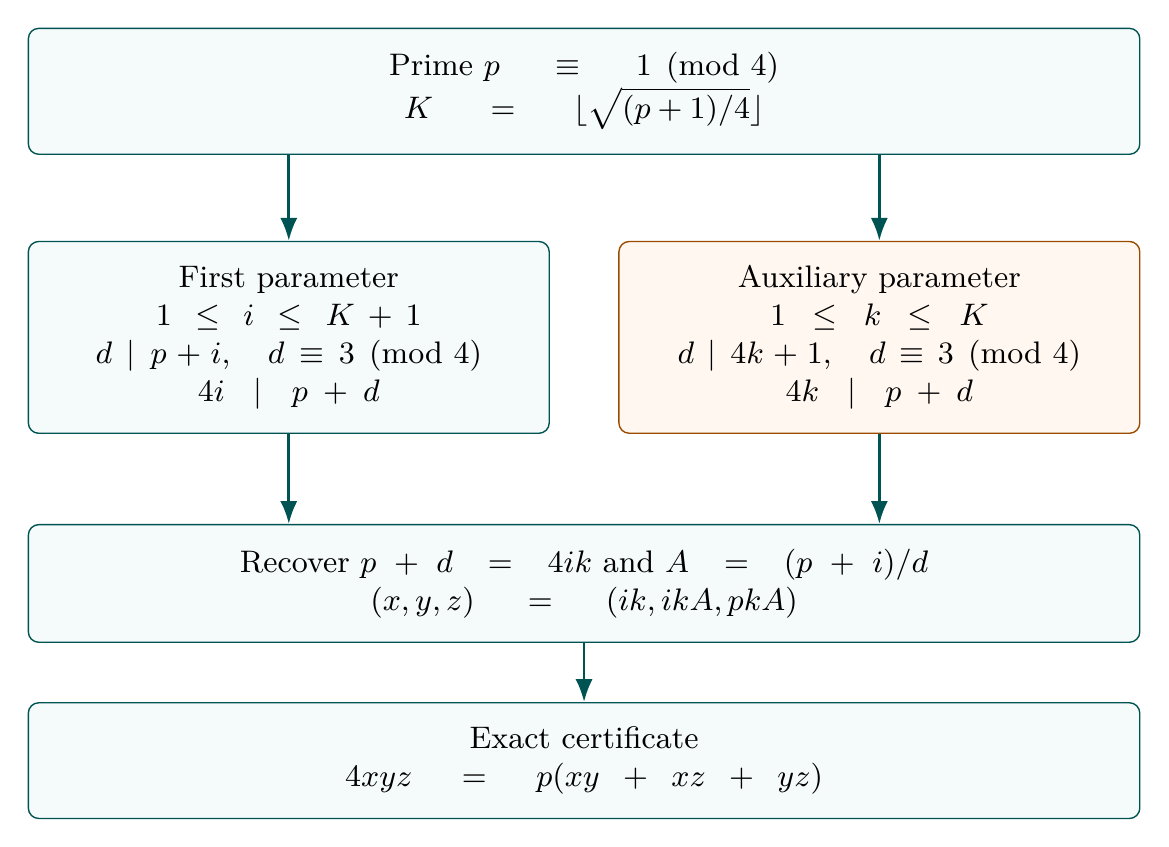
\includegraphics[width=.94\linewidth]{source-search/figures/two-channel-flow.png}
\caption{The two finite searches in Theorem~\ref{thm:twochannel}.
Every successful branch gives an exact unit-fraction certificate.}
\label{fig:twochannel}
\end{figure}

\begin{figure}[htbp]
\centering
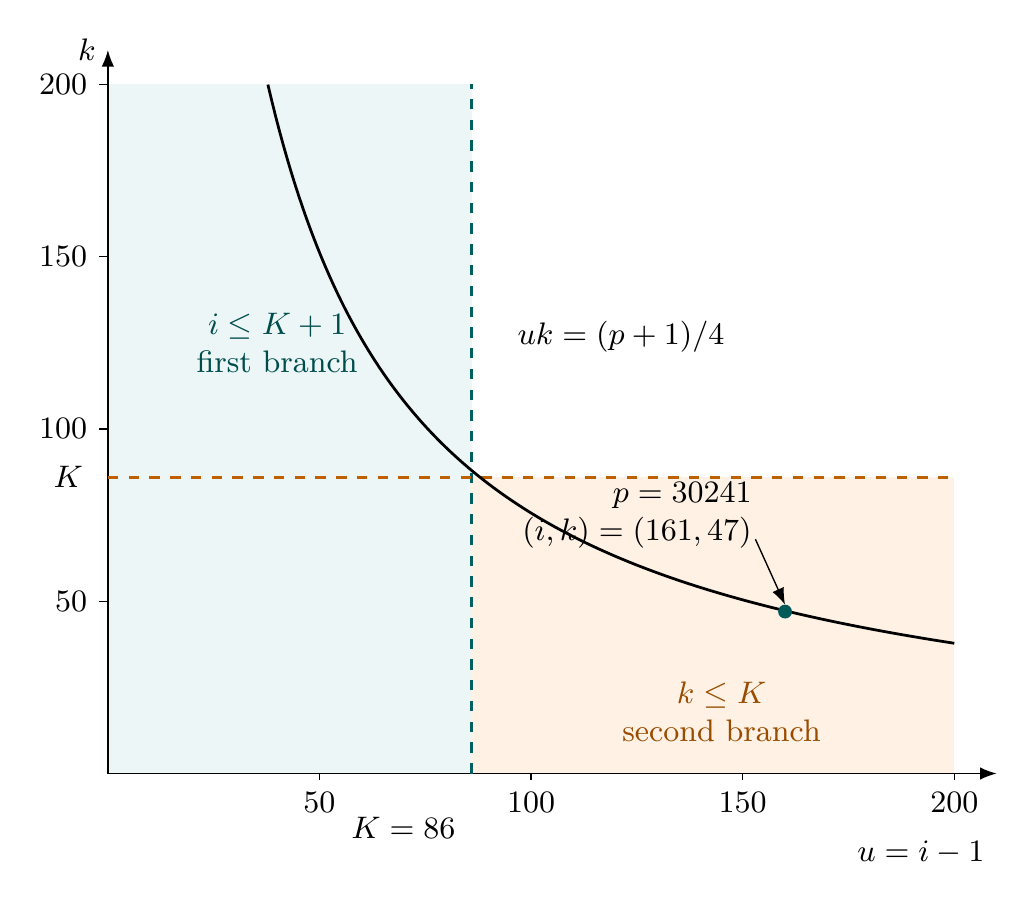
\includegraphics[width=.72\linewidth]{source-search/figures/source-hyperbola.png}
\caption{The necessary parameter bound for $p=30241$.
The shaded strips represent the two finite budgets.
The displayed witness has $i=161$ and $k=47$.
The curve is a necessary envelope, with the divisor
congruences also required for an integer point to be a witness.}
\label{fig:hyperbola}
\end{figure}

The theorem gives a complete decision procedure for the specified
$a=1$ source family using $K+1$ source indices and $K$ auxiliary
indices, with divisor enumeration at each index. The assertion that
one of these finite branches succeeds for every remaining prime is
a further nonemptiness problem. The equivalence itself imposes no
claim about its answer.


\section{Exact computation and provenance}
The standard-library program
\texttt{checks/python/source\_search.py}
checks all $1{,}289{,}653$ pairs
$(p,i)$ with $p<200000$, $p\equiv1\pmod4$ prime and
$1\le i\le\lfloor\sqrt p/2\rfloor$. Each firing certificate
is checked against the exact identity
$4xyz=p(xy+xz+yz)$. It also checks the equivalence of the two
forms of the cofactor rule and records exact rational values of
$\kappa_M$ and small large-sieve denominators. The computation
finds the single cutoff failure $30241$ in this range.
An early-terminating first-source census through $10^6$ finds
the same single failure among $39{,}175$ primes congruent to
one modulo four. These are finite ranges of verification.

The proof of Proposition~\ref{prop:30241} gives an additional
trial-division check independent of the smallest-factor table
used in the larger census. The general factor-pair criterion is
also replayed on the integers $2\le n\le300$.
The executable checks and source files are available in the
\href{https://github.com/anaxia-research/ErdosProblem1/tree/main/source-search}{research repository}.

The initial source analysis provides the prime and cofactor rules,
the fixed-depth and uniform estimates, and the starting arithmetic
large-sieve argument. This version supplies a detailed Selberg
quadratic-form lemma, records the explicit cutoff failure, and
states the complete factor-pair search. The distinct-block argument
in Section~\ref{sec:arithmeticsieve} strengthens the growing-depth
constant, and Theorem~\ref{thm:twochannel} completes the finite
source-family decision procedure.


\appendix
\section{An exact certificate for the cutoff failure}\label{app:certificate}
The following program uses trial division and integer arithmetic.
It checks that $30241$ is prime, that every source below $161$
fails, and that the first displayed witness satisfies the
unit-fraction equation.
\begin{verbatim}
from math import isqrt
p = 30241
assert all(p % d for d in range(2, isqrt(p) + 1))
for i in range(1, 161):
    n = p + i
    for q in range(1, isqrt(n) + 1):
        if n % q == 0:
            for d in (q, n // q):
                assert d % 4 != 3 or (p + d) % (4 * i) != 0
i, d = 161, 27
k, A = (p + d) // (4 * i), (p + i) // d
x, y, z = i*k, i*k*A, p*k*A
assert 4*x*y*z == p*(x*y + x*z + y*z)
\end{verbatim}

The certificate values are
\[
 p=30241,\quad i=161,\quad d=27,\quad k=47,\quad A=1126.
\]
They yield $(x,y,z)=(7567,8520442,1600414202)$.
The second search in Theorem~\ref{thm:twochannel} finds this witness
inside the budget $k\le86$.

\section{Exact checks of both complementary searches}\label{app:twochannel}
For each of the $80$ primes $p\equiv1\pmod4$ below $1000$, the
independent trial-division checker enumerates every witness with
$1\le i<p$ and compares the resulting set of triples $(i,k,d)$
with the union of the two bounded searches. Equality of these
sets is checked for all $463$ witnesses.\footnote{Equality of the
witness sets checks the completeness assertion, including overlaps
between the branches. The divisor factorizations in the large
census use a different smallest-factor implementation.}
The same program replays the integer-vector sorting step of
the large-sieve proof for small values. These computations check
the finite algebra and combinatorics used in the proofs.

\begin{center}
\begin{tabular}{@{}lr@{}}
\toprule
Verification & Count or outcome\\
\midrule
Prime inputs $p\equiv1\pmod4$ below $200000$ & $8977$\\
Source pairs at the square-root budget & $1{,}289{,}653$\\
Prime inputs $p\equiv1\pmod4$ below $10^6$ & $39{,}175$\\
Failures of the single square-root cutoff below $10^6$ & $30241$\\
Complete witness-set comparisons below $1000$ & $80$ primes\\
Witnesses in those comparisons & $463$\\
\bottomrule
\end{tabular}
\end{center}

\section{Source files and build instructions}
The email archive contains this PDF, the AMS article source,
all included proof sections, PNG figures and their TikZ sources,
exact verification reports, and the programs that reproduce them.
The principal source compiles from the archive root. Three
\texttt{pdflatex} passes resolve its references. The figures
included in the article are PNG files generated from the supplied
TikZ sources. Their generation is independent of compiling the
article itself.

The numerical constant in the density estimate and the finite
search theorem have written analytic proofs. Their verification
programs establish finite identities and enumerations. The
distribution theorems about primes used in the proof are the
stated standard inputs in analytic number theory.


\section*{Declarations}

\subsection*{Funding}
This research received no external funding.

\subsection*{Ethics approval and consent}
This work consists of mathematical proofs and exact arithmetic
computations. It involves no human participants or experimental animals.
Ethics approval and informed consent are not applicable.

\subsection*{Data and code availability}
The manuscript, source files, figures, verification programs,
and computational reports are available at
\url{https://github.com/anaxia-research/ErdosProblem1/tree/main/source-search}.

\subsection*{Declaration of AI assistance}
OpenAI ChatGPT/Codex assisted with mathematical exploration,
drafting, language editing, and verification code.
Its use included proof suggestions and computational checks.
The arguments, references, and verification procedures are
provided in the paper and repository for examination.
Responsibility for the submitted version rests with the authors.

\subsection*{Conflicts of interest}
The authors declare no conflicts of interest.

\begin{thebibliography}{99}
\bibitem{ET} C. Elsholtz and T. Tao,
Counting the number of solutions to the Erd\H{o}s--Straus equation
on unit fractions, \emph{J. Aust. Math. Soc.} 94 (2013), 50--105.
\href{https://arxiv.org/abs/1107.1010v6}{arXiv:1107.1010v6}.
\bibitem{Richert} H.-E. Richert,
\emph{Lectures on Sieve Methods}, notes by S. Srinivasan,
Tata Institute of Fundamental Research, Bombay, 1976.
\href{https://www.math.utoledo.edu/~codenth/Spring_13/3200/NT-books/Lectures_on_Sieve_Methods-Richert.pdf}{Lecture notes}.
\bibitem{HR} H. Halberstam and H.-E. Richert,
\emph{Sieve Methods}, Academic Press, London, 1974.
\bibitem{Montgomery} H. L. Montgomery,
The analytic principle of the large sieve,
\emph{Bull. Amer. Math. Soc.} 84 (1978), 547--567.
\href{https://doi.org/10.1090/S0002-9904-1978-14497-8}{doi:10.1090/S0002-9904-1978-14497-8}.
\bibitem{IK} H. Iwaniec and E. Kowalski,
\emph{Analytic Number Theory}, AMS Colloquium Publications 53,
American Mathematical Society, Providence, 2004.
\bibitem{RS} J. B. Rosser and L. Schoenfeld,
Approximate formulas for some functions of prime numbers,
\emph{Illinois J. Math.} 6 (1962), 64--94.
\href{https://doi.org/10.1215/ijm/1255631807}{doi:10.1215/ijm/1255631807}.
\bibitem{Vaughan} R. C. Vaughan,
On a problem of Erd\H{o}s, Straus and Schinzel,
\emph{Mathematika} 17 (1970), 193--198.
\href{https://doi.org/10.1112/S0025579300002886}{doi:10.1112/S0025579300002886}.
\bibitem{Dahan} B. Dahan,
\emph{Sieve dimension and search depth for the Erd\H{o}s--Straus
conjecture, $n\equiv1\pmod{24}$}, preprint, 2026.
\href{https://arxiv.org/abs/2608.24035v2}{arXiv:2608.24035v2}.
\bibitem{DahanComposite} B. Dahan,
\emph{Composite witness sieves, Kneser--Plancherel containers,
and the exponent $5/7$ for the Erd\H{o}s--Straus conjecture},
preprint, 2026.
\href{https://arxiv.org/abs/2611.08717v1}{arXiv:2611.08717v1}.
\bibitem{Trybushnyi} D. Trybushnyi,
\emph{The exponent $3/4$ for the exceptional sets of the equations
$K/n=1/x+1/y+1/z$}, preprint, 2026.
\href{https://arxiv.org/abs/2611.14167v1}{arXiv:2611.14167v1}.
\end{thebibliography}
\end{document}
